\documentclass[titlepage]{report}
\usepackage[ngerman]{babel}
\usepackage[backend=biber,style=numeric]{biblatex}
\addbibresource{literature.bib}
\usepackage{caption}
\usepackage{subcaption}
\usepackage{graphicx}
\usepackage[utf8]{inputenc}
\usepackage[T1]{fontenc}
\usepackage{url}
\usepackage{hyphenat}
\usepackage{glossaries}
\usepackage{array}
\usepackage{calc}
\usepackage{booktabs}
\usepackage{hyperref}
\usepackage{listings}
\usepackage{xcolor}
\usepackage{bytefield}
\usepackage{float}
\lstset{%
    frame=tb,
    tabsize=4,
    numbers=left,
    breaklines=true,
}
\renewcommand{\lstlistingname}{Snippet}
\renewcommand{\lstlistlistingname}{Snippets}
\makeglossaries{}
\newglossaryentry{dns}
{%
    name={DNS},
    description={},
    first={Domain Name System (DNS)},
    long={Domain Name System}
}

\newglossaryentry{http}
{%
    name={HTTP},
    description={},
    first={Hypertext Transport Protocol (HTTP)},
    long={Hypertext Transport Protocol}

}
\newglossaryentry{https}
{%
    name={HTTPS},
    description={},
    first={Hypertext Transport Protocol Secure (HTTPS)},
    long={Hypertext Transport Protocol Secure}

}
\newglossaryentry{cifs}
{%
    name={CIFS},
    description={},
    first={Common Internet File System (CIFS)},
    long={Common Internet File System}

}
\newglossaryentry{voip}
{%
    name={VoIP},
    description={},
    first={Voice Over Internet Protocol (VoIP)},
    long={Voice Over Internet Protocol}

}
\newglossaryentry{tuc}
{%
    name={TU Clausthal},
    description={},
    first={Technische Universität Clausthal},
}
\newglossaryentry{efzn}
{%
    name={EFZN},
    description={},
    first={Energie-Forschungszentrum Niedersachsen (EFZN)},
    long={Energie-Forschungszentrum Niedersachsen}
}
\newglossaryentry{rfc}
{%
    name={RFC},
    description={},
    first={Request For Comments (RFC)},
    long={Request For Comments}
}

\title{Evaluierung eines Messpunkte-Clusters für Netzwerktests auf dem
Campus der TU Clausthal}
\author{Christian, Rebischke\\
\gls{tuc}\\
Rechenzentrum\\
Email: Christian.Rebischke@tu-clausthal.de}
\begin{document}
\maketitle
\chapter*{Danksagung}
Ich bedanke mich bei dem Rechenzentrum der \gls{tuc}, insbesondere bei
Dipl.\hyp{}Math. Christian Strauf. Das Thema dieser Bachelorarbeit
beruht auf seiner Idee und war mein Ansporn mich mit diesem Thema näher
auseinanderzusetzen. Desweiteren danke ich Herrn Prof. Dr.\hyp{}Ing. Dr.
rer. nat. habil. Harald Richter für die Unterstützung aus akademischer
Seite. Besonderen Dank bekommt von mir auch die Opensource Gemeinschaft.
Ohne die harte Arbeit der Opensource Gemeinschaft würden die grundlegenden
Werkzeuge die ich zur Vollendung dieser Bachelor-Arbeit benutzt habe
nicht existieren. Darunter das Softwarepaket \LaTeX, die Zeichensoftware
\emph{Draw IO} (\url{https://www.draw.io/}) und viele weitere spannende
freiverfügbare Projekte.
\chapter*{Eidesstattliche Erklärung}
Hiermit erkläre ich an Eides statt, dass ich die vorliegende Arbeit
selbstständig und nur unter Zuhilfenahme der ausgewiesenen Hilfsmittel
angefertig habe. Sämtliche Stellen der Arbeit, die im Wortlaut oder dem
Sinn nach anderen gedruckten oder im Internet verfügbaren Werken
entnommen sind, habe ich durch genaue Quellenangaben kenntlich gemacht.
\\
\\
Clausthal-Zellerfeld, der \today
\\
\\
Christian Rebischke
\tableofcontents
\chapter*{Vorwort}
\addcontentsline{toc}{chapter}{Vorwort}
Es gibt nun seit mehr als 20 Jahren das Internet und keine Technologie
ist wohl über so kurze Zeit so alltäglich geworden. Das Internet hat es
geschafft Einzug zu erhalten in Arbeit, Privatleben und auch Forschung
und Lehre. Nahezu in allen wissenschaftlichen Diszplinen spielt das
Internet und die damit verknüpfte Informationstechnologie eine Rolle.
Sei es die Industrie 4.0 mit ihren Cyber-physischen Systemen, dem
schnellen Abgleich von DNA-Informationen über das Netz in der
angewandten Biologie, dem Sammeln von Krankheitsdaten in der Medizin
oder das Verarbeiten von Datenmengen gigantischen Ausmaßes im
Finanzsektor. All diese Beispiele sind nur möglich durch immer größere
Technologiesprünge in der Informatik und dem immer weiteren Ausbau des
Internets. Da ist es nicht verwunderlich, dass der UN-Menschenrechtsrat das
Internet zu einem Menschenrecht\cite{UNHRC} erklärt hat und umso weniger
verwunderlich ist es, dass die Vernetzung von Computersystemen auch auf
dem Campus der \gls{tuc} eine Rolle spielt,
nicht nur für Forschung und Lehre, sondern natürlich auch für den
täglichen Betrieb. Eine Schlüsselposition nimmt dabei das Rechenzentrum
der \gls{tuc} ein. Das Rechenzentrum bildet die
Basis für die Vernetzung der einzelnen Fakultäten untereinander, die
Vernetzung zwischen Fakultäten und Firmen aus der freien Wirtschaft,
sowie auch die Vernetzung zwischen der \gls{tuc}
und anderen Universitäten weltweit. Dementsprechend wichtig ist ein
stabiles Netz für den täglichen Betrieb. In dieser Bachelorarbeit widme
ich mich deshalb der technischen Umsetzung eines verteilten
Monitoring-Systems zur Überwachung der Netzwerkqualität zwischen
einzelnen Endpunkten und Kernsystemen die für einen problemlosen
Netzbetrieb nötig sind. Das Rechenzentrum der \gls{tuc} dient bei dieser
Bachelorarbeit als Auftraggeber.
\chapter*{Problemstellung}
\addcontentsline{toc}{chapter}{Problemstellung}
Das Netz der \gls{tuc} erstreckt sich über mehrere
Standorte. Teilweise liegen diese Standorte nicht in Clausthal
selbst, wie beispielsweise das \gls{efzn} in Goslar. Dementsprechend
schwierig gestaltet sich die Wartung und der Betrieb
des Netzes. So kann auf Netzeinbrüche etwa nur reaktiv
nach Meldung des Problems reagiert werden. Es existiert
zwar ein Monitoring-System, welches die Verfügbarkeit von
einzelnen Diensten überprüft, jedoch erfolgt diese Messung
nur von einem Punkt aus und gibt nur binäre Statuswerte
zurück (Dienst läuft oder Dienst läuft nicht). Dementsprechend
fehlen Informationen um die Verfügbarkeit von Diensten und
deren vollständige Funktion von mehreren Messpunkten aus
zu garantieren. Beispielsweise ist es möglich, dass ein Dienst
zwar vom zentralen Monitoring-Server aus erreichbar ist, aber
aus einem einzelnen Institut der Zugriff auf den Dienst nur
eingeschränkt oder sogar gar nicht möglich ist. Das Rechenzentrum der
\gls{tuc} bietet mehrere Kerndienste an. Dazu
gehören:
\begin{itemize}
    \item \gls{dns}
    \item Diverse Webdienste basierend auf:
    \begin{itemize}
        \item \gls{http}
        \item \gls{https}
    \end{itemize}
    \item \gls{cifs}
    \item \gls{voip}
\end{itemize}
Besonders Dienste wie \gls{dns} sind auf schnelle
Verbindungen angewiesen. Eine zu hohe Latenz zwischen einem Client und
dem Dienst führt unweigerlich zu für den Nutzer sichtbaren Konsequenzen
(zum Beispiel verzögerte Seitenaufrufe beim Web-Browsing). Noch mehr ins
Gewicht fallen Latenzen bei \gls{voip}, dort sind Latenzen
oder ein Jitter (die Varianz der Laufzeit der Datenpakete\cite{JITTERWIKI})
leicht auszumachen. Nämlich an abgehakten Telefonaten oder Rauschen in
der Leitung. Was also fehlt ist ein Netz aus verteilten Messpunkten,
dass es ermöglicht die Erreichbarkeit einzelner Dienste periodisch und
über einen längeren Zeitraum zu beobachten. Dies hätte zwei Vorteile.
Zum einen lässt sich so der Zustand des Campus-Netzwerks besser
erfassen, da Tests nicht nur von einem zentralen Monitoring-System aus
gestartet werden. Zum anderen können die gewonnenen Daten weiter
verwertet, grafisch aufbereitet und zum Beispiel für die Erstellung von
Langzeitstatistiken über die Gesundheit des Netzwerks genutzt werden.
Weiterhin könnten im Fall eines Ausfalls natürlich die zuständigen
Netzadministratoren benachrichtigt werden, im Idealfall durch gewohnte
Kommunikationswege wie Email. Mit dem Wandel von einem zentralen zu
einem dezentralen Monitoring-System entsteht allerdings auch mehr
Arbeitsaufwand. Denn auch diese Systeme müssen gewartet werden. Im
nachfolgenden Kapitel werden aus dieser Problemstellung die nötigen
Anforderungen abgeleitet und ein erster Lösungsansatz für das Problem
erstellt.
\chapter*{Technische Grundlagen}
\addcontentsline{toc}{chapter}{Technische Grundlagen}
In diesem Kapitel werden die für die Lösung des Problems nötigen
technischen Grundlagen erläutert. Darunter fallen einige wichtige
Netzwerkprotokolle, sowie eine allgemeine Einführung in
Computernetzwerke.
\section*{Netzwerkgrundlagen}
\addcontentsline{toc}{section}{Netzwerkgrundlagen}
Um auf Basis der vorangegangenen Problemstellung eine Lösung zu
erarbeiten, ist es notwendig einen groben Überblick über die Grundlagen
von Computernetzwerken zu bekommen. Als Basis dafür dient das \gls{osi}. Das
\gls{osi} ist de facto das bis heute gängige Referenzmodell, wenn es
darum geht mehrere Systeme mit einander zu vernetzen. Ein solches System
wird \emph{offenes System} genannt, wenn es den im \gls{osi}
spezifizierten Standards entspricht\cite[Siehe Abschnitt
4.1.2]{ITUOSI}. Diese \emph{offenen Systemen} sind mit einem physischen
Medium verbunden und bilden so ein Computernetzwerk. \autoref{fig:1}
zeigt eine solche Verbindung mehrerer \emph{offener Systeme}.
\begin{figure}[H]
    \centering
    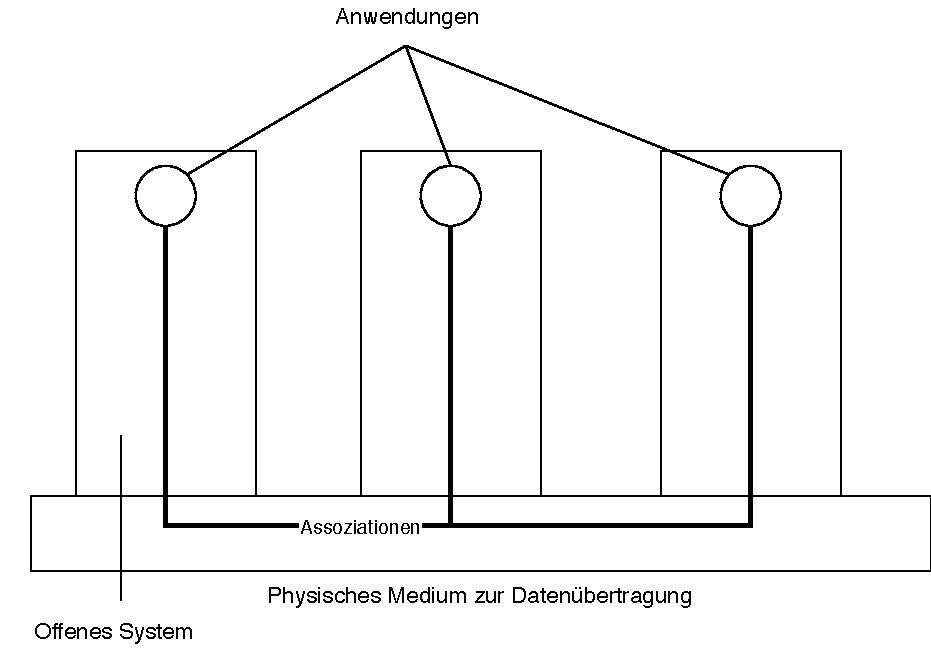
\includegraphics[width=0.8\textwidth]{figures/open_systems.pdf}
    \caption{Veranschaulichung der Assoziationen verschiedenener offener
    Systeme mit diversen Anwendungen über ein physisches Medium}\label{fig:1}
\end{figure}
Innerhalb eines dieser \emph{offener Systeme} sind sieben
Netzwerkschichten oder auch \emph{OSI-Schichten} definiert\cite[Siehe
Abschnitt 6.1.2]{ITUOSI}. Zur
Kommunikation zwischen zwei \emph{offenen Systemen} wird mindestens eine
Schicht durchlaufen, in den meisten Fällen jedoch mehrere Schichten.
\autoref{fig:2} listet alle sieben Schichten, deren Protokolle,
Einheiten und Einordnung auf. Die Funktionsweise des \gls{osi} lässt
sich am besten durch ein kurzes Beispiel erklären:

Es wird angenommen, es wird mit einem Laptop eine Website aufgerufen.
Nachfolgend wird nur der Netzverkehr zwischen dem Client und dem Server
betrachtet. Wenn der Client eine \gls{http}\hyp{}basierte Website
aufrufen möchte, sendet dieser eine \gls{http}Anfrage in Form von
\gls{http}\hyp{}Daten (Anwendungsschicht). Diese \gls{http}\hyp{}Daten
werden wiederum in ein \gls{tcp}Segment eingebettet (Transportschicht),
welches wiederum in ein \gls{ip}\hyp{}Paket eingebettet ist
(Vermittlungsschicht). Dieses \gls{ip}\hyp{}Paket enthält die Adresse
des Empfängers und wird ebenfalls eingebettet in einen
Ethernet\hyp{}Frame (Sicherungsschicht), welcher wiederum in Form von
Bits über ein Netzwerkkabel übertragen wird (Bitübertragungsschicht).
Dieses Matrjoschka\hyp{}ähnliche Gebilde wird dann über das physische
Medium versendet und der Empfänger packt es angefangen bei der
Bitübertragungsschicht von unten nach oben wieder aus.

\textbf{Anmerkung}: Es handelt sich hierbei um eine starkvereinfachte
Darstellung. In der Realität kommen diverse andere Faktoren dazu, wie in
etwa:
\begin{itemize}
    \item Das Auflösen eines Hostnamen mit \gls{dns}
    \item Das Routing über \gls{ip}
    \item Der Aufbau einer Session mit \gls{tcp}
    \item \ldots
\end{itemize}
\begin{figure}[H]
    \centering
    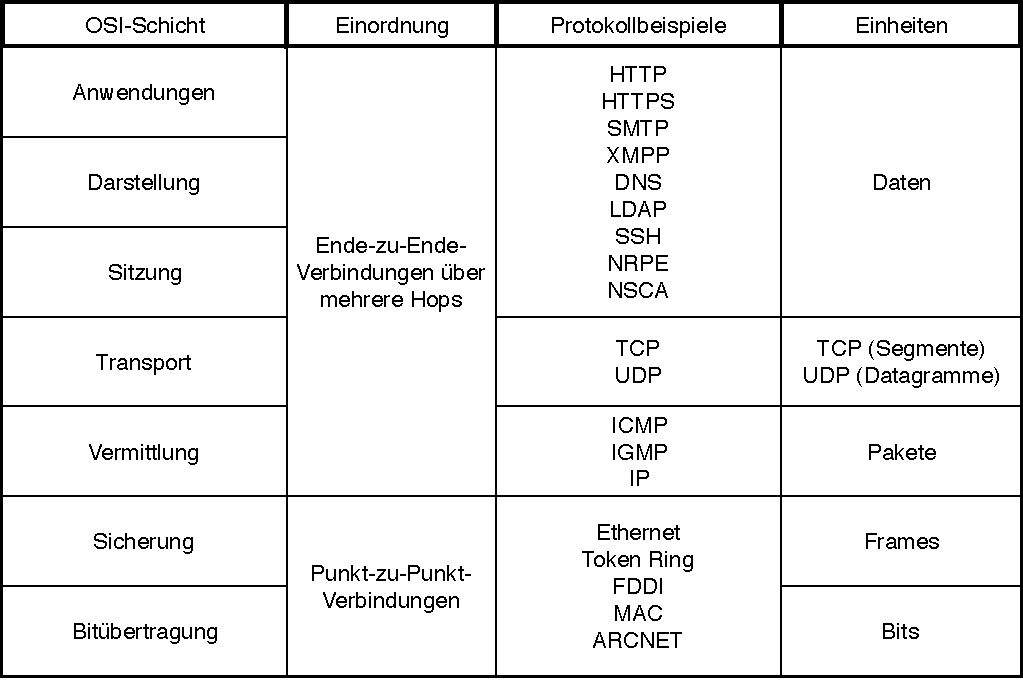
\includegraphics[width=0.8\textwidth]{figures/osi.pdf}
    \caption{Das OSI-Schichtenmodell mit Protokollbeispielen und
    verwendeten Einheiten}\label{fig:2}
\end{figure}
\section*{\glsfirst{dns}}
\addcontentsline{toc}{section}{\glsfirst{dns}}
Aus Erfahrungen mit dem Internetvorgänger \gls{arpanet} wurde
abgeleitet, dass ein manuelles Eingeben von \gls{ip}\hyp{}adressen mit
steigender Anzahl von Knoten im Netzwerk immer unübersichtlicher wurde.
Hinzukommend sind \gls{ip}\hyp{}Adressen für den Menschen schwer zu
merken. Mit dieser Problemstellung als Grundlage arbeitete der Ingenieur
Peter Mockapetris an einem ersten Lösungsansatz: \glsfirst{dns}.
Bei \gls{dns} handelt es sich um einen mehr als 20 Jahre alten
Verzeichnisdienst, welcher über das gleichnamige Protokoll, für Menschen
merkbare Internetadressen auf \gls{ip}\hyp{}Adressen abbildet.
\gls{dns} wurde erstmalig im Jahr 1983 in den beiden \glspl{rfc}
\gls{rfc} 882\cite{RFC0882} und \gls{rfc} 883\cite{RFC0883} beschrieben.
Damals befanden sich die \gls{dns}\hyp{}Einträge, die Abbildungen von
lesbarer Adresse auf \gls{ip}\hyp{}Adresse, noch verteilt auf
allen Servern des frühen Internets und wurden von der \gls{nic} verwaltet
und mit dem Dateiübertragungsprotokoll \gls{ftp}
synchronisiert\cite{RFC1034}. In der damaligen Zeit stellte sich dies
als ein Flaschenhals für das Internet heraus, da die Anzahl der Server
im Netzwerk exponentiell zunahm. Deshalb wurden nur vier Jahre später
Überarbeitungen von \gls{dns} veröffentlicht. Diese Überarbeitungen
wurden in den \glspl{rfc} \gls{rfc} 1034 und \gls{rfc} 1035 erläutert
und bilden die Grundlage für \gls{dns} wie es heute bekannt ist und auch
eingesetzt wird. Der heutige Ansatz verläuft dezentraler als es damals
der Fall gewesen ist. Anstatt die \gls{dns}\hyp{}Einträge auf allen
Knoten des Internets zu verteilen und zentral von der \gls{nic} aus zu
steuern, existieren heute mehrere hierarchische Verwaltungsebenen. Dazu
wird der \gls{fqdn} hierarchisch gegliedert. Ein Beispiel für einen
\gls{fqdn} ist beispielsweise \emph{akira.rz.tu-clausthal.de}. Die
\autoref{fig:3} veranschaulicht, die Gliederung dieses \gls{fqdn} in die
einzelnen Bestandteile.
\begin{figure}[H]
    \centering
    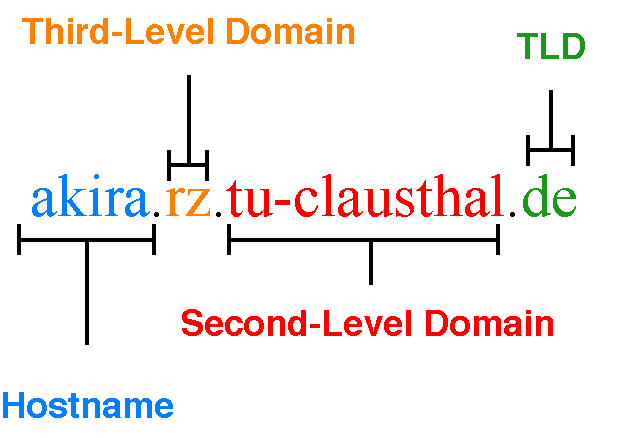
\includegraphics[width=0.5\textwidth]{figures/dnsname.pdf}
    \caption{Bestandteile eines \gls{fqdn} mit optionalem Hostname und Third-Level
    Domain}\label{fig:3}
\end{figure}
Eine Angabe des Hostname oder einer Third-Level
Domain ist optional. Es können auch weitere Domains hinzugefügt werden.
So ist auch eine Sixth-Level Domain möglich. Die Maximale Anzahl der
Subdomains ist in keinem der \gls{dns} \glspl{rfc} spezifiziert. Deshalb
ist die maximale Anzahl abhängig vom \gls{dns}\hyp{}Server der die
Domains ausliefert. Nach \gls{rfc} 1035 ist die maximale Länge eines
\gls{fqdn} aber auf 255 Bytes begrenzt\cite[siehe Section
2.3.4]{RFC1035}, was die maximale Anzahl von Subdomains zumindest stark
einschränkt. Der Begriff Subdomain umfasst alle Domains unter der
\gls{tld}. \glspl{fqdn} sind nicht nur hierarchisch strukturiert, sondern
unterliegen zusätzlich einer Baumstruktur. Dessen Wurzel ist die
\emph{Root Domain}, meistens symbolisiert durch einen einfachen Punkt.
Eine Ebene direkt darunter sind die \glspl{tld} diese
werden in der Regel von den \glspl{nic} einzelner Länder verwaltet. Von
Ländern verwaltete \glspl{tld} haben meist Länderabkürzungen wie
\emph{de} (Deutschland), \emph{jp} (Japan) oder \emph{cn} (Volksrepublik
China). Es existieren aber auch militärische oder akademische
\glspl{tld} wie \emph{edu} und \emph{mil}. In Deutschland ist die DENIC eG
verantwortlich für Domains mit \emph{de}\hyp{}Endung.
In den letzten 5 Jahren kamen auch noch neue \glspl{tld} hinzu, welche
nicht an Länder geknüpft sind. Darunter fallen Markennamen wie
\emph{BMW}, \emph{Audi} oder \emph{Deutschepost} oder markenfreie Namen
wie \emph{academy}, \emph{fun} oder \emph{house}\cite{NEWTLDLIST}. Die
Vergabe der \glspl{tld} verlief direkt über die \gls{icann}. Der jeweilige
Käufer ist dann Eigentümer der jeweiligen \gls{tld}. Ein Eigentümer
einer \gls{tld} kann dann beliebig viele Subdomains erstellen für den
Eigenbedarf, diese weiterverkaufen oder gar verschenken. Weitere
wichtige Elemente des \gls{dns}\hyp{}Protokolls sind \emph{Name Server}
und \emph{Resolver}\cite[Siehe Section 2.4]{RFC1034}.
\emph{Name Server} sind Server Programme, welche
Informationen zu der Baumstruktur enthalten. Ergo halten \emph{Name
Server} Domain\hyp{}\gls{ip}\hyp{}\hyp{}Tabellen für ihre
hierarchische Ebene vor. Wenn kein Eintrag zu dem angefragten \gls{fqdn}
existiert wird der nächsthöhere \gls{dns}\hyp{}Server gefragt. An
oberster Stelle stehen 13 \emph{Root Nameserver
Server}\cite{ROOTNAMESERVER}. Die \emph{Root
Name Server} umfassen die Namen und \gls{ip}\hyp{}Adressen aller
\emph{Name Server} die für die \gls{tld} verantwortlich sind.
\emph{Resolver} übernehmen die Rolle des Clients, sie senden
\gls{dns}\hyp{}Anfragen an \emph{Name Server}. Diese
Anfragen erfolgen in den meisten Fällen über \gls{udp} an den Zielport
53\cite[Siehe Section 4.2.1]{RFC1035}. Es ist allerdings auch \gls{dns}
über \gls{tcp} spezifiziert\cite[Siehe Section 4.2.2]{RFC1035}.
\section*{\glsfirst{http}}
\addcontentsline{toc}{section}{\glsfirst{http}}
\glsfirst{http} ist ein auf \gls{tcp}/\gls{ip} aufbauendes
Datenübertragungsprotokoll, welcher auf der Andwendungsschicht des
\gls{osi} operiert. Der am meisten verbreiteste Anwendungszweck für das
Protokoll ist das Ausliefern von Webseiten über Port 80. \gls{http}
wurde erstmals im Jahre 1996 als \gls{rfc} 1945 spezifiziert, nach dem
es bereits fast 6 Jahre im Internet im Einsatz gewesen
war\cite{RFC1945}. Im Laufe der Jahre kamen dann weitere Versionen,
sowie diverse Erweiterungen für das Protokoll hinzu. Darunter
Erweiterungen für Kompression (um die Datenübertragungsrate zu erhöhen),
Verschlüsselung, Caching und Authentifikation. Seit 2015 ist die
aktuelle Version \gls{http}/2, welche in \gls{rfc} 7540 standardisiert
wird\cite{RFC7540}. \gls{http} ist ein zustandsloses Protokoll,
dementsprechend werden mehrere Anfragen getrennt von einander und ohne
Kontext zu einander bearbeitet. Es wird keine Session aufgebaut und
keine Sitzungsinformationen verwaltet. Sitzungsinformationen können
aber zusätzlich durch \emph{Cookies} übertragen werden. \emph{Cookies}
ergänzen den \gls{http}\hyp{}Header um Sitzungsinformationen, dadurch
ist dann eine genaue Zuordnung möglich. Zur Interaktion mit dem Server
besitzt \gls{http} mehrere Methoden. Die häufigsten sind:
\begin{description}
    \item[GET] für einfache Anfragen
    \item[POST] um Informationen wie beispielsweise Logindaten an den
        Server zu senden.
    \item[HEAD] ist ähnlich wie \textbf{GET} mit dem Unterschied, dass
        der Server bei einer Antwort keinen Inhalt mitliefert.
\end{description}
Weitere Methoden sind \textbf{DELETE}, \textbf{PUT} und \textbf{OPTIONS}
die hier nicht weiter erläutert werden, da diese nur für eine
\gls{restapi} verwendet werden.
Im \autoref{lst:1} ist eine \gls{http}\hyp{}Anfrage mit Antwort und
Verbindungsaufbau an den Host \emph{http://tu-clausthal.de}
visualisiert. Die eigentliche \gls{http}\hyp{}Anfrage beginnt ab Zeile 5
und ended in Zeile 9. Aus Zeile 5 wird ersichtlich, dass es sich um die
Version 1.1 von \gls{http} handelt und der Client via \emph{GET} den
Index der Seite \emph{tu-clausthal.de} (siehe Zeile 6) anfragt. Zeile 7
übermittelt den Namen und Version der Software mit dem diese
\gls{http}\hyp{}Anfrage gesendet worden ist und Zeile 8 definiert,
welche Mediatypen in einer Antwort erlaubt sind\cite{RFC2616}. Ab Zeile
10 beginnt dann die Antwort des Servers. Dort wird das Protokoll und die
Version nochmal bestätigt und in diesem Beispiel ein Statuscode
hinzugefügt (301 weist daraufhin, dass der Inhalt der Seite verschoben
worden ist und an einem neuen Ort liegt (siehe Zeile 13)). Dazu wird auf
eine neue \gls{url} verwiesen. Die \gls{url} dient als Pfadangabe zur
gewünschten Ressource oder Information. Bei \gls{http} haben diese
Pfadangaben den Präfix \emph{http://}. Zeile 11 gibt
das aktuelle Datum, die Uhrzeit und die Zeitzone an und Zeile 12 die
Software des Servers und deren Version. Die Zeilen 14,15 und 16
enthalten die Information, dass der Server diverse Encodings unterstützt
(zum Beispiel Kompression mit dem Kompressionsalgorithmus \emph{gzip}),
die Länge des übermittelten Inhalts und der Typ des Inhalts sowie dessen
Zeichenkodierung. Die Zeilen 18 bis 21 enthalten dann den übermittelten
Inhalt. Hier gekürzt dargestellt.
\begin{lstlisting}[caption={Eine HTTP-Anfrage an
http://tu-clausthal.de},label={lst:1}]
* Rebuilt URL to: http://tu-clausthal.de/
*   Trying 2001:638:605:20:1::2...
* TCP_NODELAY set
* Connected to tu-clausthal.de (2001:638:605:20:1::2) port 80 (#0)
> GET / HTTP/1.1
> Host: tu-clausthal.de
> User-Agent: curl/7.59.0
> Accept: */*
>
< HTTP/1.1 301 Moved Permanently
< Date: Fri, 11 May 2018 23:48:50 GMT
< Server: Apache/2.2.22 (Ubuntu)
< Location: http://www.tu-clausthal.de/
< Vary: Accept-Encoding
< Content-Length: 235
< Content-Type: text/html; charset=iso-8859-1
<
<!DOCTYPE HTML PUBLIC "-//IETF//DTD HTML 2.0//EN">
<html><head>
[...]
</body></html>
* Connection #0 to host tu-clausthal.de left intact
\end{lstlisting}
\section*{\glsfirst{https}}
\addcontentsline{toc}{section}{\glsfirst{https}}
Bei \gls{https} handelt es sich um das Protokoll \gls{http} mit einer
zusätzlichen Schicht zur Verschlüsselung und Herstellung von
Datenintegrität. Dafür wird das Verschlüsselungsprotokoll \gls{tls}
benutzt, teilweise auch noch unter der Bezeichnung \gls{ssl} bekannt.
Wobei anzumerken ist, dass \gls{ssl} der Name des Vorgängers ist.
Für den Verbindungsaufbau wird bei \gls{https} standardmäßig
Port 433 benutzt\cite[Siehe Section 2.3]{RFC2818}. Als
\gls{url}\hyp{}Präfix dient \emph{https://}. Bei der Verschlüsselung und
Herstellung der Datenintegrität bleibt die eigentliche
\gls{http}\hyp{}Syntax intakt, ergo findet eine Verschlüsselung der
einzelnen \gls{http}\hyp{}Pakete statt. Dazu verschickt der Client beim
Verbindungsaufbau über Port 433 ein \emph{TLS ClientHello} an den
Server, daraufhin wird dann der \gls{tls}\hyp{}Handshake initiiert.
Dieser Handshake beinhaltet die Überprüfung der Integrität des Servers
unter Betrachtung des \gls{tls}\hyp{}Zertifikats. Das Zertifikat ist
nichts anderes als ein öffentlicher Schlüssel, welcher mit einer
digitalen Signatur einer Zertifizierungsstelle beglaubigt worden ist.
Der Client besitzt eine Datenbank mit gültigen Zertifizierungsstellen
und vergleicht so das signierte Zertifikat des Servers mit dem
Zertifikat einer Zertifizierungsstelle. Wurden keine Mängel
festgestellt, beispielsweise ein abgelaufenes Zertifikat oder eine
fremde Zertifizierungsstelle, geht der Client davon aus, dass der Server
die Identität besitzt, die er vorgibt zu haben. Dies ist in so fern
problematisch, als dass in der Vergangenheit wiederholt bei
Zertifizierungsstellen eingebrochen worden ist und private Schlüssel zum
erstellen von gültigen Zertifikaten gestohlen worden
sind\cite{PRIVATEKEYSSTOLEN}. Nach der Integritätsprüfung folgt dann der
eigentliche Aufbau einer verschlüsselten Verbindung. Für den Aufbau
existieren im Augenblick zwei mögliche Verfahren. Zum Einen der
\gls{rsa}\hyp{}Handshake und zum Anderen der
Diffie\hyp{}Hellman\hyp{}Handshake\cite{TLS}. Beim
\gls{rsa}\hyp{}Handshake wird vom Client ein symmetrischer Schlüssel
erzeugt, dieser wird dann mit dem öffentlichen Schlüssel des Servers
verschlüsselt und dem Server mitgeteilt. Der Server entschlüsselt den
symmetrischen Schlüssel unter Zuhilfenahme seines privaten Schlüssels.
Damit ist eine sichere Verbindung aufgebaut und der Client und Server
sind in der Lage sich mit dem symmetrischen Schlüssel
verschlüsselte Nachrichten zu senden. Beim
Diffie\hyp{}Hellman\hyp{}Handshake dagegen werden die öffentlichen
Schlüssel beider Gesprächspartner ausgetauscht und mit dem jeweiligen im
Besitz befindlichen privaten Schlüssel ein gemeinsamer symmetrischer
Schlüssel berechnet. Dieser symmetrische Schlüssel verlässt im Gegensatz
zum \gls{rsa}\hyp{}Handshake niemals den Server oder Client. Außerdem
ist es möglich für jede Session einen neuen flüchtigen symmetrischen Key
zu erzeugen, dies wird ermöglicht in dem bei jeder neuen Session ein
neues Schlüsselpaar erzeugt wird. Ergo ist der
Diffie\hyp{}Hellman\hyp{}Handshake als sicherer anzusehen, da der
gemeinsame symmetrische Schlüssel niemals übertragen wird (auch nicht
verschlüsselt) und neue Sessions immer mit einem neuen Schlüssel
versehen werden. Letzteres ermöglicht \gls{pfs}.  Durch \gls{pfs} ist es
einem Angreifer mit einem aktuellen privaten Schlüssel nicht möglich
ältere aufgezeichnete Verbindungen zu entschlüsseln.
\section*{\glsfirst{cifs}}
\addcontentsline{toc}{section}{\glsfirst{cifs}}
\gls{cifs} ist ein von der Firma Microsoft 1996 eingeführtes
Datentransferprotokoll auf Basis von \gls{smb}\cite{SMBWIKI} und
\gls{netbios} über \gls{tcp}/\gls{ip}. Das Protokoll ist nicht nur auf
Dateitransfer beschränkt, sondern kann auch für Druckerfreigaben,
Windows-RPC (ein von Microsoft eingeführtes Protokoll um Code aus der
Ferne auszuführen) und den NT-Domänendienst (Ein von Microsoft
eingeführter Dienst zur Authentifizierung von Computern und Nutzern)
verwendet werden. Für die in dem vorherigen Kapitel genannte
Problemstellung ist allerdings nur der Dateitransfer via \gls{smb} von
Relevanz. Im Gegensatz zu \gls{http} ist \gls{cifs} ein
sessionbehaftetes Protokoll. Der \gls{cifs}\hyp{}Server ordnet also
jeder Verbindung eine Sitzung zu die einem Client genau zugeordnet
werden kann, darüber sind diverse Operationen möglich wie
Authentifizierung, Verschlüsselung oder \emph{Locking}\cite[S.
16]{MSSMB}. Beim \emph{Locking} wird der Zugriff auf eine Datei
beschränkt um deren Korruption zu vermeiden, welche passieren kann wenn
mehrere Nutzer auf die gleiche Datei schreiben. Um dies zu verhindern
setzt der \gls{cifs}\hyp{}Server ein \emph{Lock} auf diese Datei und
lässt nur einen Client in diese Datei schreiben. Der eigentliche
Transfer der Dateien wird mit \gls{tcp} vor Korruption geschützt.
Die von der \gls{iana} für \gls{cifs} vergebene Portnummer ist:
445\cite[S. 19]{MSSMB}. Desweiteren hat \gls{tcp} den Vorteil, dass es
\emph{full-duplex} ist. \emph{Full-duplex} bedeutet, dass \gls{tcp} in
der Lage ist gleichzeitig Daten zu empfangen und zu senden.
\autoref{fig:4} zeigt den Aufbau eines solchen \gls{smb}\hyp{}Pakets mit
\gls{tcp}\hyp{}Header. Der Header beginnt mit einem Byte aus Nullen und
der anschließenden Länge des \gls{smb}\hyp{}Pakets. Danach kommt in 32
Byte Blöcken die eigentliche Nachricht. Die Länge des Pakets wird als
drei Byte Integer in \emph{Network Byte Order} repräsentiert\cite[S.
21]{MSSMB}. \emph{Network Byte Order} entspricht dem \emph{Big Endian
Format} bei dem das höchstwertige Byte zu erst gespeichert wird.
\begin{figure}[h]
    \centering
    \begin{bytefield}{32}
        \bitheader{0-31}\\
        \bitbox{8}{Null-Byte} & \bitbox{24}{Länge des SMB-Pakets}\\
        \bitbox{32}{SMB Nachricht}\\
        \bitbox{32}{\ldots}
    \end{bytefield}
    \caption{Aufbau eines \gls{smb}\hyp{}Pakets}\label{fig:4}
\end{figure}
\section*{\glsfirst{voip}}
\addcontentsline{toc}{section}{\glsfirst{voip}}
\chapter*{Herleitung eines Lösungsansatzes}
\addcontentsline{toc}{chapter}{Herleitung eines Lösungsansatzes}
\section*{Anforderungsanalyse}
\addcontentsline{toc}{section}{Anforderungsanalyse}
Nachfolgend werden die ermittelten funktionalen und nichtfunktionalen
Anforderungen erläutert. Funktionale Anforderungen stellen das
``eigentliche Systemverhalten und die jeweiligen Funktionen des zu
erstellenden Produkts''\cite[S. 20]{BPSE} dar, also die grundlegenden
Aufgaben der Software im Bezug auf die Problemstellung. Die
nichtfunktionalen Anforderungen dagegen sind besonders. Sie umfassen
Anforderungen wie Sicherheit, nachträgliche Erweiterbarkeit,
Testbarkeit, also Anforderungen die erst nach der Entwicklung
mess\hyp{} oder testbar werden\cite[S. 292]{SNFA}. Um die funktionalen
und nichtfunktionalen Anforderungen besser einordnen zu können, werden
folgende Schlüsselwörter zum Kennzeichnen für Anforderungen nach
\gls{rfc} 2119\cite{RFC2119} definiert:
\begin{description}
    \item[MUSS] ist eine absolute Anforderung an die Software. Alle
        Anforderungen die mit \textbf{MUSS} markiert sind,
        \textbf{MÜSSEN} implementiert werden.
    \item[DARF NICHT] beschreibt eine negative Anforderung. Demnach eine
        Anforderung die auf keinen Fall implementiert werden darf.
    \item[SOLL] ist eine Anforderung die implementiert werden
        \textbf{SOLLTE} aber nicht \textbf{MUSS}. Dies ist der Fall bei
        Anforderungen die aus nachvollziehbaren Gründen nicht
        implementiert werden.
    \item[MUSS NICHT] ist das Gegenteil von \textbf{MUSS}. Es
        handelt sich hier um Anforderungen die vermieden werden sollten.
    \item[KANN] ist eine Anforderung die implementiert werden
        \textbf{KANN}. Diese Art von Anforderungen sind
        zusätzliches Extra und nicht nötig für die Grundfunktion der
        Software.
\end{description}
\textbf{Anmerkung}: Das \gls{rfc} 2119 ist im Original in Englisch. Ich
habe mich zur übersetzung der Schlüsselwörter auf die Übersetzung der
Schweizer Firma Adfinis SyGroup AG gestützt\cite{RFC2119DE}.
\subsection*{Funktionale Anforderungen}
\addcontentsline{toc}{subsection}{Funktionale Anforderungen}
\begin{center}
\begin{tabular}{p{0.7\textwidth-\tabcolsep}>{\raggedleft\arraybackslash}p{0.3\textwidth-\tabcolsep}}\toprule
    \textbf{FA1: Überwachung von \gls{dns} } & \textbf{Priorität: MUSS} \\\midrule
	\multicolumn{2}{p{\textwidth-\tabcolsep}}{%
        Die Software muss die Erreichbarkeit mehrerer
        \gls{dns}\hyp{}Server überprüfen können. Ebenfalls muss die
        Latenz einer \gls{dns}\hyp{}Anfrage gemessen werden können.}\\bottomrule
\end{tabular}
\end{center}
\begin{center}
\begin{tabular}{p{0.7\textwidth-\tabcolsep}>{\raggedleft\arraybackslash}p{0.3\textwidth-\tabcolsep}}\toprule
    \textbf{FA2: Überwachung von \gls{http} } & \textbf{Priorität: MUSS} \\\midrule
	\multicolumn{2}{p{\textwidth-\tabcolsep}}{%
        Die Software \textbf{MUSS} die Erreichbarkeit mehrerer
        \gls{http}\hyp{}Server überprüfen können. Ebenfalls muss die
        Latenz einer \gls{http}\hyp{}Anfrage gemessen werden können.}\\\bottomrule
\end{tabular}
\end{center}
\begin{center}
\begin{tabular}{p{0.7\textwidth-\tabcolsep}>{\raggedleft\arraybackslash}p{0.3\textwidth-\tabcolsep}}\toprule
    \textbf{FA3: Überwachung von \gls{https} } & \textbf{Priorität: MUSS} \\\midrule
	\multicolumn{2}{p{\textwidth-\tabcolsep}}{%
        Die Software \textbf{MUSS} die Erreichbarkeit mehrerer
        \gls{https}\hyp{}Server überprüfen können. Ebenfalls muss die
        Latenz einer \gls{https}\hyp{}Anfrage gemessen werden können.}\\\bottomrule
\end{tabular}
\end{center}
\begin{center}
\begin{tabular}{p{0.7\textwidth-\tabcolsep}>{\raggedleft\arraybackslash}p{0.3\textwidth-\tabcolsep}}\toprule
    \textbf{FA4: Überwachung von \gls{cifs} } & \textbf{Priorität: SOLL} \\\midrule
	\multicolumn{2}{p{\textwidth-\tabcolsep}}{%
    Die Software \textbf{MUSS} die Zeit messen können, die vergeht
    zwischen einer \gls{cifs}-Abfrage und der Antwort von einem
    \gls{cifs}-Server}\\\bottomrule
\end{tabular}
\end{center}
\begin{center}
\begin{tabular}{p{0.7\textwidth-\tabcolsep}>{\raggedleft\arraybackslash}p{0.3\textwidth-\tabcolsep}}\toprule
    \textbf{FA5: Zeitmessung von \gls{voip}-Abfragen } & \textbf{Priorität: KANN} \\\midrule
	\multicolumn{2}{p{\textwidth-\tabcolsep}}{%
    Die Software \textbf{MUSS} die Zeit messen können, die vergeht
    zwischen einer \gls{voip}-Abfrage und der Antwort von einem
    \gls{voip}-Server}\\\bottomrule
\end{tabular}
\end{center}
\begin{center}
\begin{tabular}{p{0.7\textwidth-\tabcolsep}>{\raggedleft\arraybackslash}p{0.3\textwidth-\tabcolsep}}\toprule
    \textbf{FA6: Speicherung von Performance-Daten in einer Datenbank } & \textbf{Priorität: MUSS} \\\midrule
	\multicolumn{2}{p{\textwidth-\tabcolsep}}{%
        Das System \textbf{MUSS} die gesammelten Performance-Daten
        zur weiteren Auswertung an eine Datenbank übertragen.}\\\bottomrule
\end{tabular}
\end{center}
\begin{center}
\begin{tabular}{p{0.7\textwidth-\tabcolsep}>{\raggedleft\arraybackslash}p{0.3\textwidth-\tabcolsep}}\toprule
    \textbf{FA7: Grafische Aufbereitung } & \textbf{Priorität: MUSS} \\\midrule
	\multicolumn{2}{p{\textwidth-\tabcolsep}}{%
        Die vom System zur Datenbank gesendeten Performance-Daten
        \textbf{MÜSSEN} für die Administratoren grafisch in Form von
        Graphen aufbereitet werden.
        Diese Graphen \textbf{MÜSSEN} via Port 80 (\gls{http})
        und Port 443 (\gls{https}) erreichbar sein.
        }\\\bottomrule
\end{tabular}
\end{center}
\begin{center}
\begin{tabular}{p{0.7\textwidth-\tabcolsep}>{\raggedleft\arraybackslash}p{0.3\textwidth-\tabcolsep}}\toprule
    \textbf{FA8: Bandbreitenmessung } & \textbf{Priorität: MUSS} \\\midrule
	\multicolumn{2}{p{\textwidth-\tabcolsep}}{%
        Das System \textbf{MUSS} in der Lage sein Bandbreitenmessungen anhand des
        Durchsatzes vorzunehmen.
                }\\\bottomrule
\end{tabular}
\end{center}
\subsection*{Nichtfunktionale Anforderungen}
\addcontentsline{toc}{subsection}{Nichtfunktionale Anforderungen}
\begin{center}
\begin{tabular}{p{0.7\textwidth-\tabcolsep}>{\raggedleft\arraybackslash}p{0.3\textwidth-\tabcolsep}}\toprule
    \textbf{NFA1: Wahl der Programmiersprache} & \textbf{Priorität: MUSS} \\\midrule
	\multicolumn{2}{p{\textwidth-\tabcolsep}}{%
        Das System \textbf{MUSS} in einer dem Rechenzentrum der
        \gls{tuc} gängigen Programmiersprache entwickelt werden.
        Folgende Programmiersprachen werden im Rechenzentrum der
        \gls{tuc} täglich benutzt:
        \begin{itemize}
            \item Python
            \item Bash
            \item PHP
            \item Javascript
        \end{itemize}
    }\\\bottomrule
\end{tabular}
\end{center}
\begin{center}
\begin{tabular}{p{0.7\textwidth-\tabcolsep}>{\raggedleft\arraybackslash}p{0.3\textwidth-\tabcolsep}}\toprule
    \textbf{NFA2: Niedrige Beschaffungskosten} & \textbf{Priorität: SOLL} \\\midrule
	\multicolumn{2}{p{\textwidth-\tabcolsep}}{%
    Die Hardware des Systems \textbf{SOLL} möglichst günstig in der Beschaffung
    sein.
    }\\\bottomrule
\end{tabular}
\end{center}
\begin{center}
\begin{tabular}{p{0.7\textwidth-\tabcolsep}>{\raggedleft\arraybackslash}p{0.3\textwidth-\tabcolsep}}\toprule
    \textbf{NFA3: Native 1 Gigabit Ethernet Schnittstelle} & \textbf{Priorität: SOLL} \\\midrule
	\multicolumn{2}{p{\textwidth-\tabcolsep}}{%
    Die Hardware des Systems \textbf{SOLL} über eine native 1 Gigabit
    Ethernet Schnittstelle verfügen.
    }\\\bottomrule
\end{tabular}
\end{center}
\begin{center}
\begin{tabular}{p{0.7\textwidth-\tabcolsep}>{\raggedleft\arraybackslash}p{0.3\textwidth-\tabcolsep}}\toprule
    \textbf{NFA4: Sicherheit} & \textbf{Priorität: MUSS} \\\midrule
	\multicolumn{2}{p{\textwidth-\tabcolsep}}{%
        Das System \textbf{MUSS} sicher konzipiert sein.
        Alle Übertragungen müssen \textbf{MÜSSEN} mit gängigen
        als sicher eingestuften Algorithmen verschlüsselt sein,
        ausgenommen die Testverbindungen, die keine Verschlüsselung
        vorsehen.
        }\\\bottomrule
\end{tabular}
\end{center}
\section*{Systemarchitektur}
\addcontentsline{toc}{section}{Systemarchitektur}

\begin{figure}[H]
    \centering
    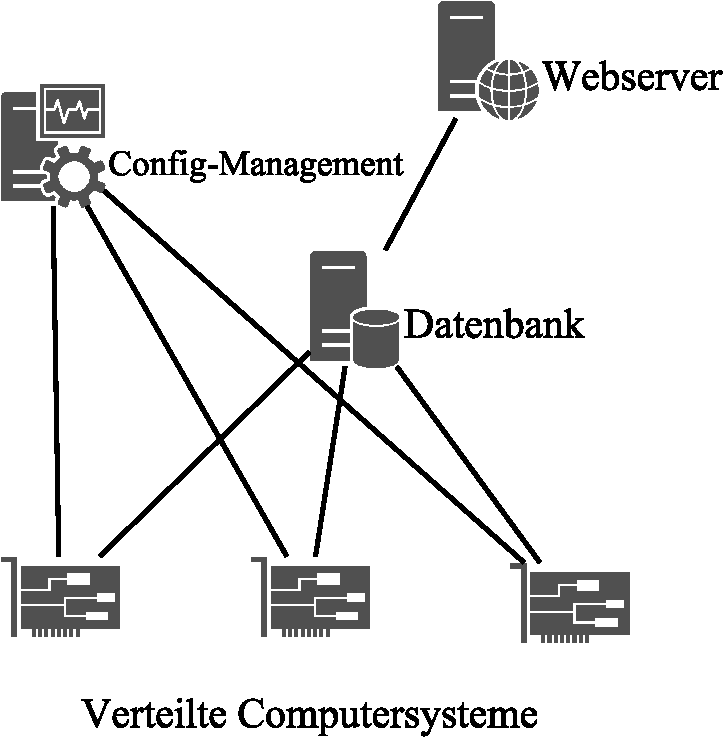
\includegraphics[width=0.5\textwidth]{figures/network.pdf}
    \caption{Übersicht der einzelnen Komponenten der zu entwickelnden
    Systeme}\label{fig:5}
\end{figure}
\chapter*{Projektumsetzung}
\addcontentsline{toc}{chapter}{Projektumsetzung}
\chapter*{Fazit}
\addcontentsline{toc}{chapter}{Fazit}
\nocite{*}
\printbibliography{}
\lstlistoflistings{}
\listoffigures
\printglossary{}
\end{document}
